
% LaTeX Beamer file automatically generated from DocOnce
% https://github.com/hplgit/doconce

%-------------------- begin beamer-specific preamble ----------------------

\documentclass{beamer}

\usetheme{red_plain}
\usecolortheme{default}

% turn off the almost invisible, yet disturbing, navigation symbols:
\setbeamertemplate{navigation symbols}{}

% Examples on customization:
%\usecolortheme[named=RawSienna]{structure}
%\usetheme[height=7mm]{Rochester}
%\setbeamerfont{frametitle}{family=\rmfamily,shape=\itshape}
%\setbeamertemplate{items}[ball]
%\setbeamertemplate{blocks}[rounded][shadow=true]
%\useoutertheme{infolines}
%
%\usefonttheme{}
%\useinntertheme{}
%
%\setbeameroption{show notes}
%\setbeameroption{show notes on second screen=right}

% fine for B/W printing:
%\usecolortheme{seahorse}

\usepackage{pgf,pgfarrows,pgfnodes,pgfautomata,pgfheaps,pgfshade}
\usepackage{graphicx}
\usepackage{epsfig}
\usepackage{relsize}

\usepackage{fancybox}  % make sure fancybox is loaded before fancyvrb

\usepackage{fancyvrb}
%\usepackage{minted} % requires pygments and latex -shell-escape filename
%\usepackage{anslistings}
%\usepackage{listingsutf8}

\usepackage{amsmath,amssymb,bm}
%\usepackage[latin1]{inputenc}
\usepackage[T1]{fontenc}
\usepackage[utf8]{inputenc}
\usepackage{colortbl}
\usepackage[english]{babel}
\usepackage{tikz}
\usepackage{framed}
% Use some nice templates
\beamertemplatetransparentcovereddynamic

% --- begin table of contents based on sections ---
% Delete this, if you do not want the table of contents to pop up at
% the beginning of each section:
% (Only section headings can enter the table of contents in Beamer
% slides generated from DocOnce source, while subsections are used
% for the title in ordinary slides.)
\AtBeginSection[]
{
  \begin{frame}<beamer>[plain]
  \frametitle{}
  %\frametitle{Outline}
  \tableofcontents[currentsection]
  \end{frame}
}
% --- end table of contents based on sections ---

% If you wish to uncover everything in a step-wise fashion, uncomment
% the following command:

%\beamerdefaultoverlayspecification{<+->}

\newcommand{\shortinlinecomment}[3]{\note{\textbf{#1}: #2}}
\newcommand{\longinlinecomment}[3]{\shortinlinecomment{#1}{#2}{#3}}

\definecolor{linkcolor}{rgb}{0,0,0.4}
\hypersetup{
    colorlinks=true,
    linkcolor=linkcolor,
    urlcolor=linkcolor,
    pdfmenubar=true,
    pdftoolbar=true,
    bookmarksdepth=3
    }
\setlength{\parskip}{0pt}  % {1em}

\newenvironment{doconceexercise}{}{}
\newcounter{doconceexercisecounter}
\newenvironment{doconce:movie}{}{}
\newcounter{doconce:movie:counter}

\newcommand{\subex}[1]{\noindent\textbf{#1}}  % for subexercises: a), b), etc

%-------------------- end beamer-specific preamble ----------------------

% Add user's preamble




% insert custom LaTeX commands...

\raggedbottom
\makeindex

%-------------------- end preamble ----------------------

\begin{document}

% endif for #ifdef PREAMBLE



% ------------------- main content ----------------------



% ----------------- title -------------------------

\title{Education for the future}

% ----------------- author(s) -------------------------

\author{Morten Hjorth-Jensen\inst{1,2}
\and
Anders Malthe-Sørenssen\inst{1}}
\institute{Department of Physics, University of Oslo\inst{1}
\and
Department of Physics and Astronomy, Michigan State University, USA\inst{2}}
% ----------------- end author(s) -------------------------

\date{September 2 2015,
% <optional titlepage figure>
}

\begin{frame}[plain,fragile]
\titlepage
\end{frame}

\begin{frame}[plain,fragile]
\frametitle{This talk is about how we perceive the role of education; present and future}

\begin{block}{}

\begin{itemize}
\item \textbf{Research-based education}, from undergraduate studies to a PhD: \href{{http://www.mn.uio.no/fysikk/english/research/groups/computational/index.html}}{The Computational Physics group at the University of Oslo} as example

\item Future challenges and directions
\end{itemize}

\noindent
\end{block}
\begin{block}{Takeaway message }
A successful research program cannot be disconnected from education and vice versa
\end{block}
\end{frame}

\begin{frame}[plain,fragile]
\frametitle{The role of computations, from education to society}

\pause
\begin{block}{}
\textbf{Computations of almost all systems in science are central to our
basic understanding of nature and technological advances}.
\end{block}

\begin{block}{Examples }
\begin{itemize}
\item \textbf{Nanotech and Materials}: quantum physical systems in nanotechnology; characteristics of new materials; semi-conductor devices and quantum computers 

\item \textbf{The smallest particles in nature}: subatomic physics at its smallest length scale

\item \textbf{And the largest}: simulating galaxies and the evolution of the universe

\item \textbf{Life science}: cancer treatment and how the brain works

\item \textbf{Geosciences}: predicting climate changes and this week's weather, simulating natural disasters

\item \textbf{Finance}: assessing risk in the insurance and financial industry

\item and many many more
\end{itemize}

\noindent
\end{block}
\end{frame}

\begin{frame}[plain,fragile]
\frametitle{Modeling and computations as a way to enhance algorithminc thinking}

\pause
\begin{block}{}
\textbf{Algorithm} :
A set of instructions to solve a problem.
% A finite set of unambiguous instructions that, given some set of initial condit#ions, can be performed in a prescribed sequence to achieve a certain goal.
\end{block}

<<<<<<< HEAD
\begin{block}{Algorithmic thinking: }

=======
\begin{block}{}
\textbf{Algorithmic  thinking as a way to} :
>>>>>>> 5fc06d357468ca5ec59d2d3ed0179709275f8f00
\begin{itemize}
\item Enhances instruction-based teaching

\item Introduces research-based teaching  from day one

\item Triggers further insights in math and other disciplines

<<<<<<< HEAD
\item Emphasizes validation and verification of scientific results, and integrates ethics

\item Ensures good working practices from day one!
=======
\item Validation and verification of scientific results, with the possibility to emphasize ethical aspects as well. Version control is central

\item Good working practices from day one
>>>>>>> 5fc06d357468ca5ec59d2d3ed0179709275f8f00
\end{itemize}

\noindent
\end{block}
\end{frame}

\begin{frame}[plain,fragile]
<<<<<<< HEAD
\frametitle{What does computing mean?}

\begin{block}{}

\textbf{Computing means solving scientific problems using computers. It covers numerical as well as symbolic computing. Computing is also about developing an understanding of the scientific process by enhancing the algorithmic thinking when solving problems.}
\end{block}
=======
\frametitle{What do we mean with computing?}

\begin{block}{}

\textbf{Computing means solving scientific problems using computers. It covers numerical as well as symbolic computing. Computing is also about developing an understanding of the scientific process by enhancing algorithmic thinking when solving problems.}
>>>>>>> 5fc06d357468ca5ec59d2d3ed0179709275f8f00


\begin{block}{Computing competence is about: }

\begin{itemize}
\item derivation, verification, and implementation of algorithms

\item understanding what can go wrong with algorithms

\item overview of important, known algorithms

\item understanding how algorithms are used to solve complicated problems

\item reproducible science and ethics

\item algorithmic thinking for gaining deeper insights about scientific problems
\end{itemize}

\noindent
<<<<<<< HEAD
All these elements (and many more) aid students in maturing and gaining a better understanding of the scientific process.
=======
All these elements (and many more) aid students in maturing and gaining a better understanding of the scientific process \emph{per se}.  
>>>>>>> 5fc06d357468ca5ec59d2d3ed0179709275f8f00
\end{block}
\end{frame}

\begin{frame}[plain,fragile]
\frametitle{Computing and research-based education}

\pause
\begin{block}{}
A computational approach allows us to introduce research concepts and engage students in research from \emph{day one}.
\end{block}
\begin{block}{How do we define research-based education? }
It is fully integrated with a direct participation in actual research and builds upon established
knowledge and insights about scientific methods.

\shortinlinecomment{hpl 1}{ Think this is unclear...better to just phrase it orally? }{ Think this is unclear...better }
\end{block}
\end{frame}

\begin{frame}[plain,fragile]
\frametitle{Research-based education}

\begin{block}{What should the education contain? }

\begin{itemize}
\item Theory + experiment + simulation is the norm in research and industry

\item Modeling of real, complex systems with no simple answers

\item Insight and understanding of fundamental principles and laws

\item Visualization, presentation, discussion, interpretation, and critical analysis of results

\item Development of a sound ethical attitude to own and other's work

\item Enhanced reasoning about the scientific method
\end{itemize}

\noindent
This is what we do in the \href{{http://www.mn.uio.no/fysikk/english/research/groups/computational/index.html}}{Computational Physics group at UiO}!
\end{block}
\end{frame}

\begin{frame}[plain,fragile]
\frametitle{\href{{http://www.mn.uio.no/fysikk/english/research/groups/computational/index.html}}{Computational Physics group at UiO}; our visions}

\begin{columns}
\column{0.6\textwidth}
\begin{block}{}
<<<<<<< HEAD
A particular strength of physics students is their ability to \textbf{pose and
solve problems} that combine \textbf{physical insights} with \textbf{mathematical tools}
and now also \textbf{computational skills}. This provides a unique combination
of applied and theoretical knowledge and skills. These features are invaluable
for the development of multi-disciplinary educational and research programs.
=======
A particular strength of physics students is their ability to pose and
solve problems that combine physical insights with mathematical
and  computational skills. This provides a unique combination
of applied and theoretical knowledge and skills. These features are invaluable 
for the development of multi-disciplinary educational and research programs for future challenges. 
>>>>>>> 5fc06d357468ca5ec59d2d3ed0179709275f8f00
\end{block}

\column{0.4\textwidth}
% inline figure
\centerline{
\includegraphics[width=1.0\linewidth]{fig-future/computer_nerd2.jpg}}



\end{columns}
\end{frame}

\begin{frame}[plain,fragile]
\frametitle{We develop a social and scientific learning environment}

\begin{block}{}
<<<<<<< HEAD
The main aim is that students should realize their own potentials and creative power

\begin{itemize}
 \item Students come with different dreams, ambitions, aspirations and topics they wish to study, our approach is to tailor the education to all these aspects
=======
\begin{itemize}
\item \textbf{The main aim is that students should realize their own potentials and creative power}
\begin{itemize}

 \item Students come with different dreams, ambitions, aspirations and topics they wish to study, our approach is to tailor the education to all these, an possibly more, aspects
>>>>>>> 5fc06d357468ca5ec59d2d3ed0179709275f8f00

 \item Our motto: foster students who are better than their supervisors - that's progress!

 \item Students and teachers help each other

<<<<<<< HEAD
 \item Students with different backgrounds and needs can thrive socially and scientifically

 \item No competing environment, but a drive and enthusiam for sharing and developing knowledge
=======
 \item No competing environment but a drive and enthusiam in sharing and developing new knowledge

 \item This creates an enviroment where students with different backgrounds and needs can thrive socially and scientifically

\end{itemize}

\noindent
\item \textbf{Takeaway message: Developing a collaborative educational environment is central for multi-disciplinary research projects to succeed}
>>>>>>> 5fc06d357468ca5ec59d2d3ed0179709275f8f00
\end{itemize}

\noindent
\end{block}
\end{frame}

\begin{frame}[plain,fragile]
\frametitle{We develop a social and scientific learning environment}

\begin{block}{}
\begin{itemize}
\item We target bachelor, MSc and PhD students

\item Project-oriented work where students develop and mature their own ideas, with an individually tailored approach to each student

\item Office space with desktops to every student and large common room for recreational activities (meals, gaming, movies)

\item Many students collaborate on similar  thesis topics and \href{{http://www.dn.no/talent/2014/06/12/Utdannelse/sommervikar-ble-toppforsker}}{publish in top scientific journals}
\end{itemize}

\noindent
\end{block}
\end{frame}

\begin{frame}[plain,fragile]
\frametitle{Features of the Computational Physics group}

\begin{block}{}
\begin{itemize}
\item Our students have made significant contributions to  the \href{{http://www.mn.uio.no/english/about/collaboration/cse/}}{Computing in Science Education}  (UiO education prize in 2011) by developing exercises and participating in educational projects at the MN faculty

\item Our students have also developed educational \href{{http://www.mn.uio.no/fysikk/om/aktuelt/aktuelle-saker/2015/realfagsapper.html}}{tools and applications for understanding complicated physical problems}

\item A group of PhD students is now developing \href{{https://github.com/CINPLA/ibvcse}}{new textbooks for Computational Life Science}

\item 2005-2015: $> 60$ students have finalized their master's theses and 60\% have continued with PhD studies

\item Many students don't want to leave the group after finishing their studies
\end{itemize}

\noindent
\end{block}
\end{frame}

\begin{frame}[plain,fragile]
\frametitle{Investing in equipment for students}

\begin{block}{Using research funds for visualization tools }


% inline figure
\centerline{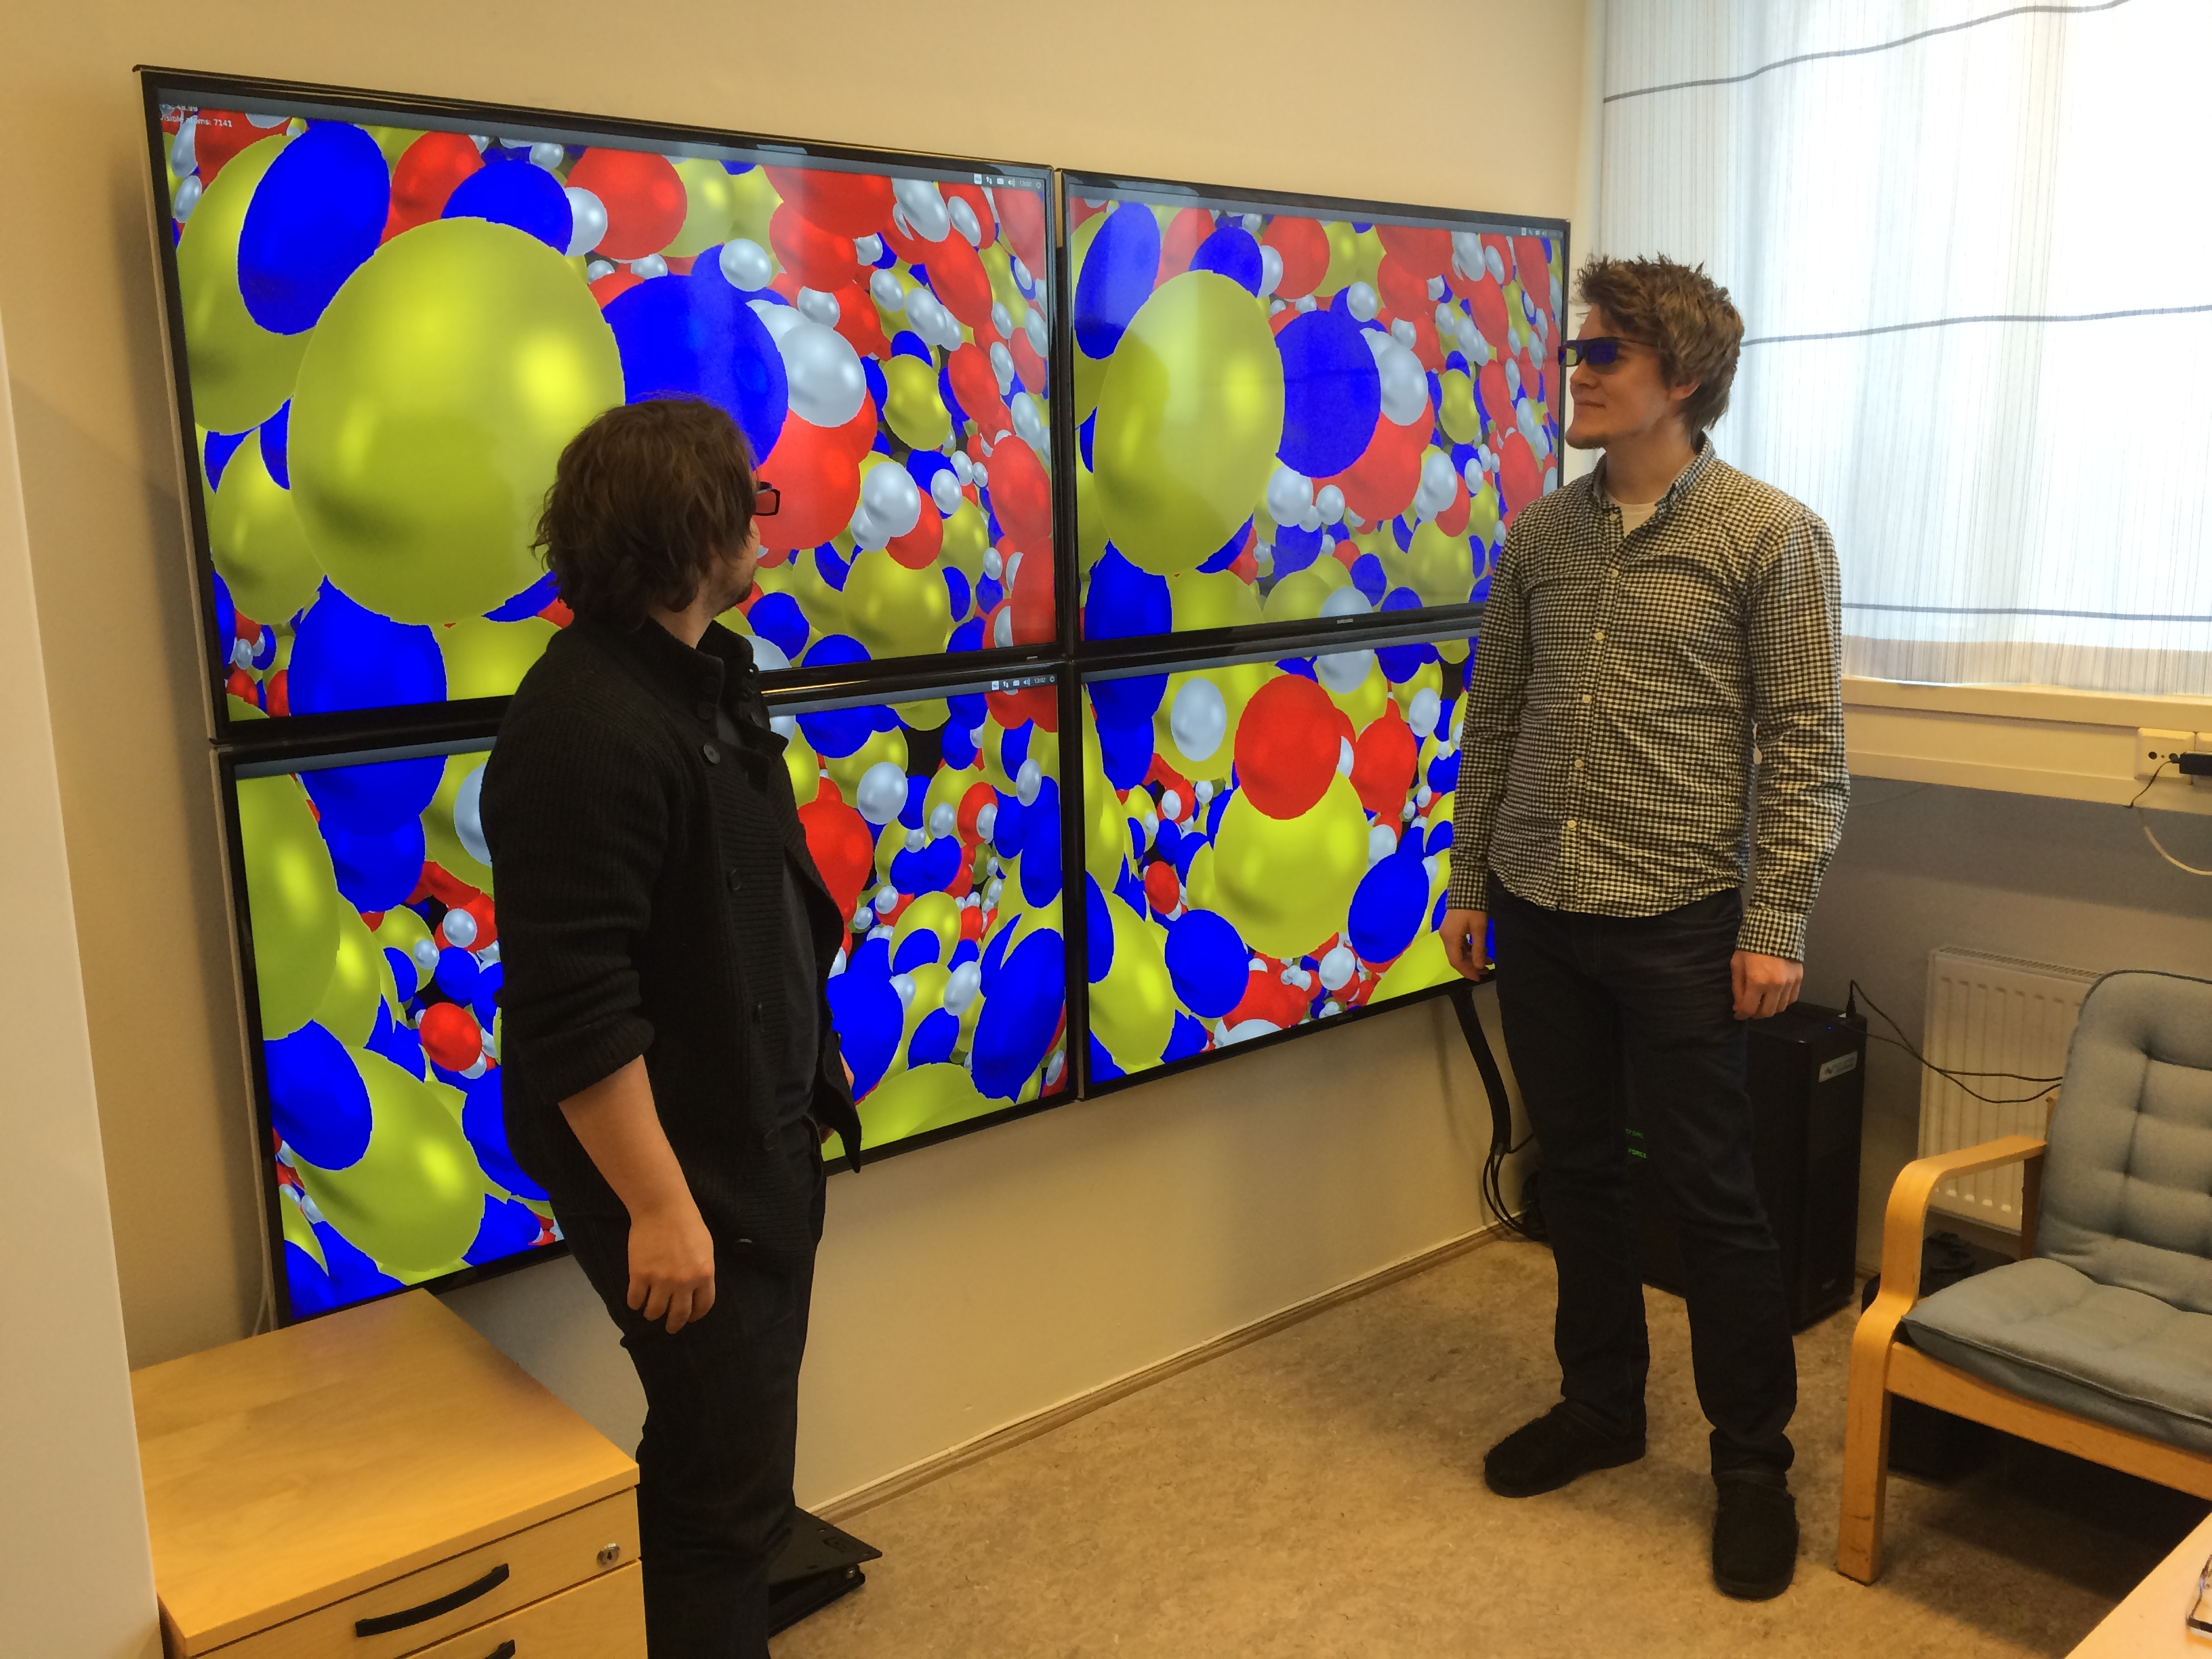
\includegraphics[width=0.7\linewidth]{fig-future/visualize.jpg}}



\end{block}
\end{frame}

\begin{frame}[plain,fragile]
\frametitle{Building a supercomputing cluster}

\begin{block}{We got (for free) the old supercomputer at UiO (TITAN) }


% inline figure
\centerline{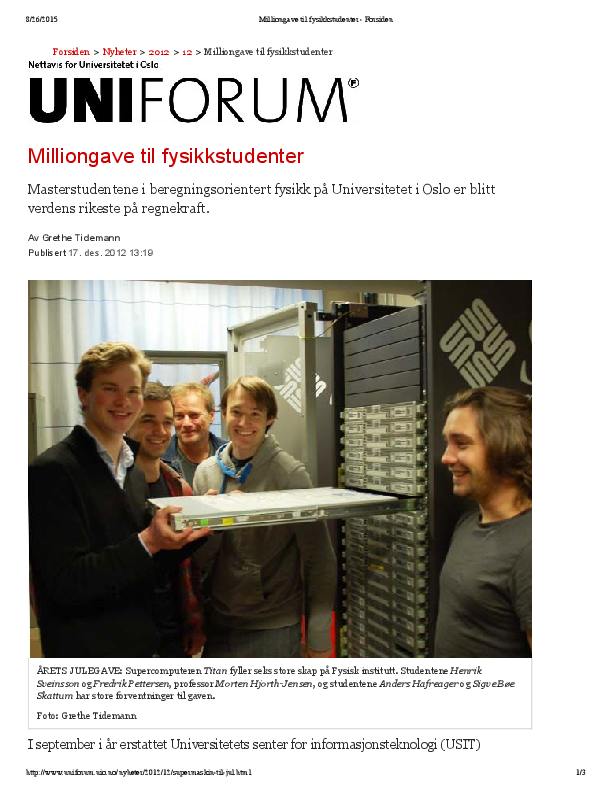
\includegraphics[width=0.7\linewidth]{fig-future/uniforum-0.png}}



\end{block}
\end{frame}

\begin{frame}[plain,fragile]
\frametitle{Undergraduate student publishes in PNAS}

\begin{block}{Using research funds for visualization tools }


% inline figure
\centerline{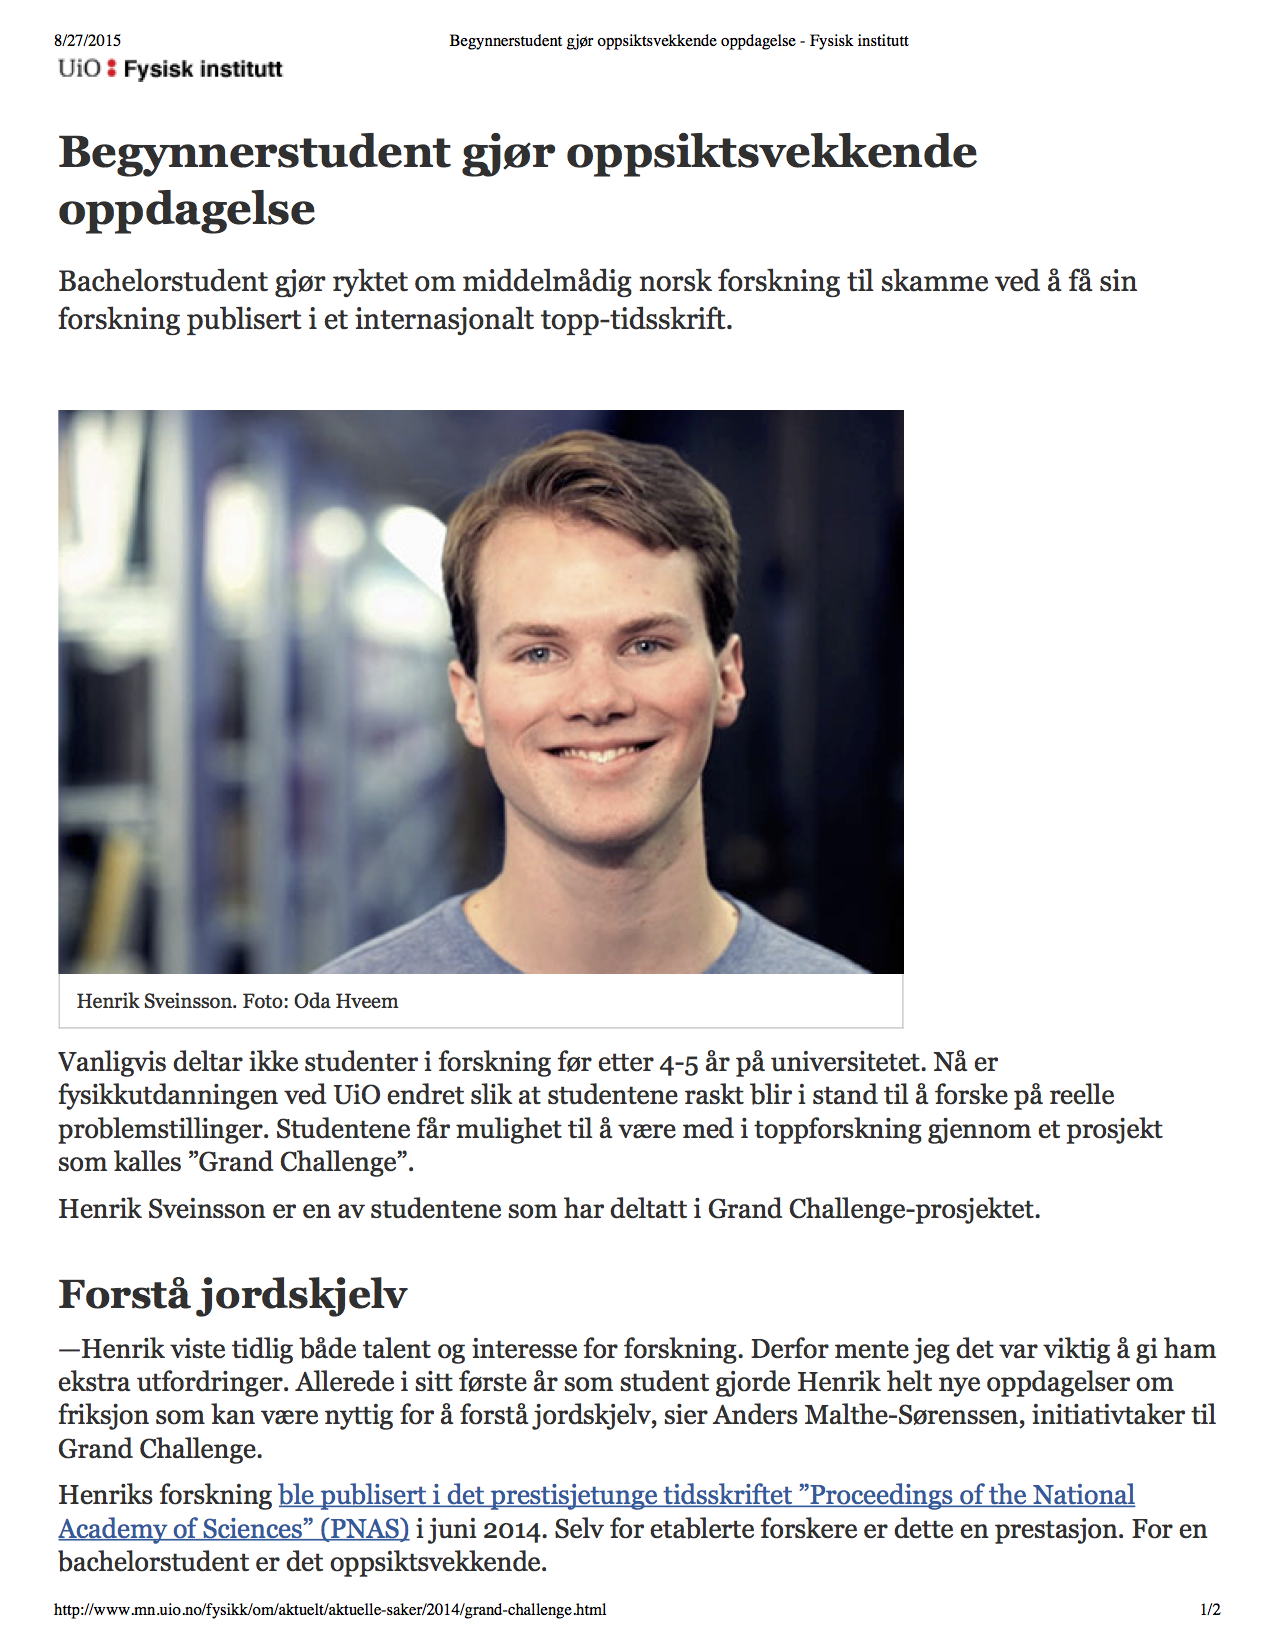
\includegraphics[width=0.7\linewidth]{fig-future/pnas.png}}



\end{block}
\end{frame}

\begin{frame}[plain,fragile]
\frametitle{Multiscale modeling is the big open research question in the 21st century}

\begin{block}{}
\begin{itemize}
\item Present and future problems, unlike traditional
  science and engineering, involve complex systems with many distinct
  physical processes

\item The wide open research topic of this century, both in industry and at universities, is how to effectively couple processes across different length and energy scales

\item Progress will rely on a \emph{multi-disciplinary} approach
\end{itemize}

\noindent
\end{block}

\begin{block}{}
We need to foster candidates with the right
multi-disciplinary background and computational thinking!
\end{block}
\end{frame}

\begin{frame}[plain,fragile]
\frametitle{Examples of large scale simulations}

<<<<<<< HEAD
\begin{block}{Fluid dynamical simulations central in air industry.  Typical university courses which are taught address the physics of the lower left corner. }
=======
\begin{block}{Fluid dynamical simulations central in air industry.  }
>>>>>>> 5fc06d357468ca5ec59d2d3ed0179709275f8f00


% inline figure
\centerline{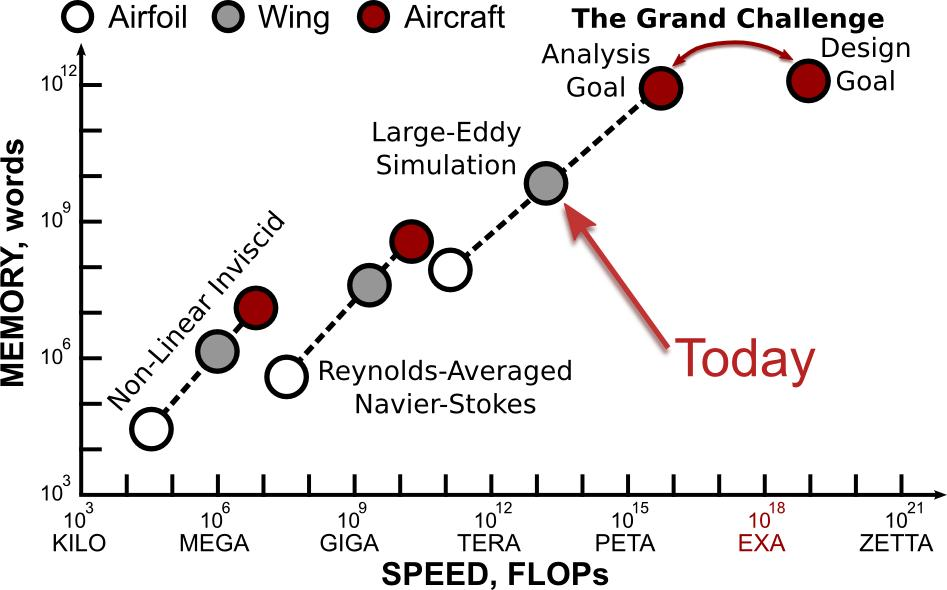
\includegraphics[width=0.6\linewidth]{fig-future/fig10.jpg}}


\end{block}
\end{frame}

\begin{frame}[plain,fragile]
\frametitle{Testing plane wings via massive numerical simulations}

\begin{block}{}
Fluid dynamical simulations central in air industry, wings tested.


% inline figure
\centerline{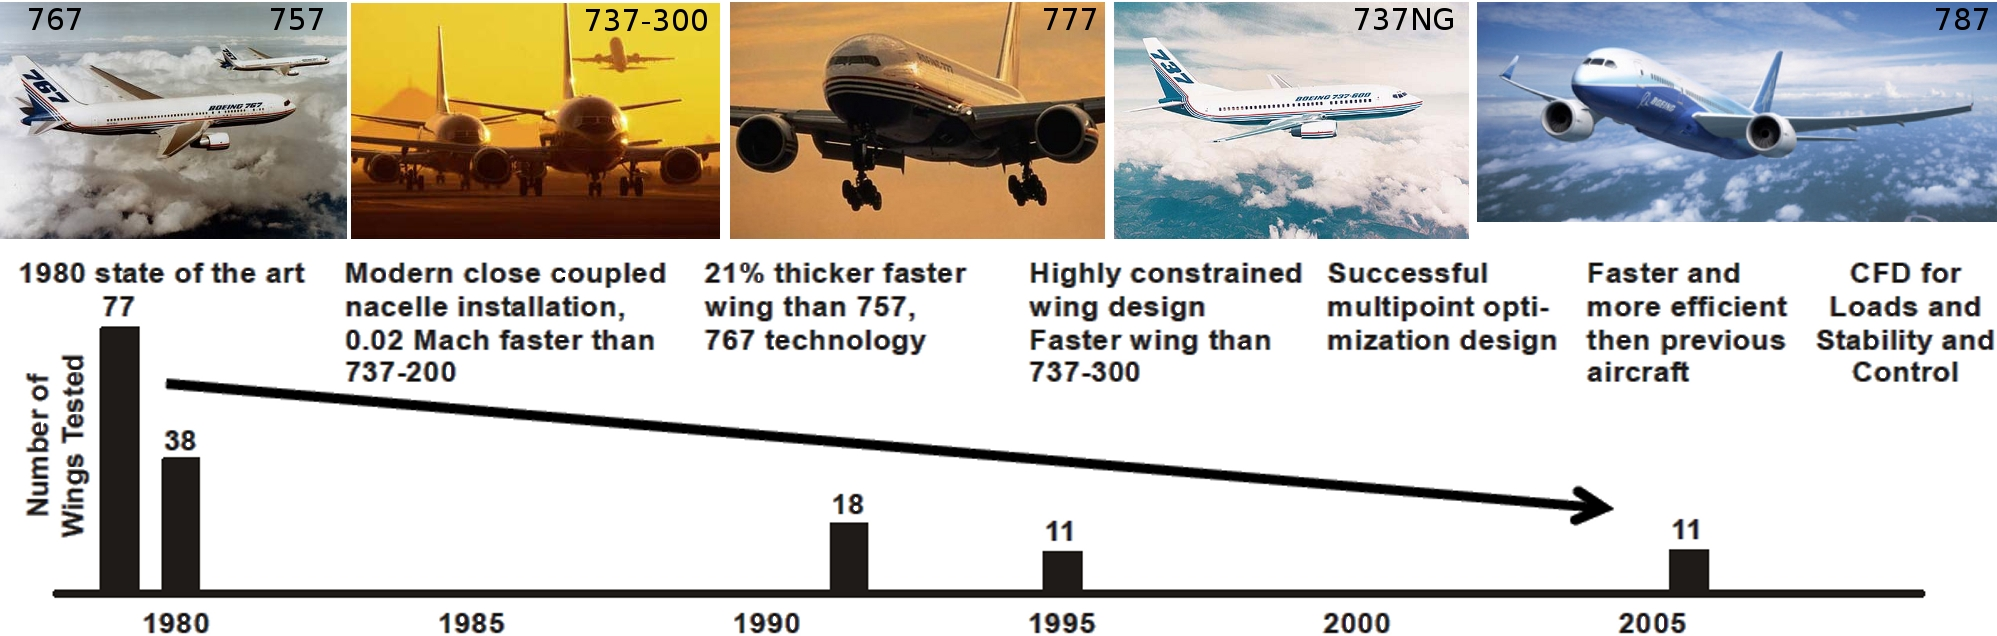
\includegraphics[width=1.0\linewidth]{fig-future/fig8.jpg}}


\end{block}
\end{frame}

\begin{frame}[plain,fragile]
\frametitle{The future: A new type of students}

\begin{block}{}
<<<<<<< HEAD
We need to educate the next generation of
science students with the knowledge, skills, and values needed to pose
and solve current and new scientific, technological and societal
challenges.
\end{block}
\begin{block}{}
This will lay the foundation for cross-disciplinary
educational, research and innovation activities. It will contribute to building a common cross-disciplinary
approach to key strategic initiatives, with examples like \emph{Energy, Materials, Life Science, and Enabling Technologies}.
\end{block}

\shortinlinecomment{hpl 2}{ Repetitions on this slide, lengthy text - better to just phrase this in the delivery }{ Repetitions on this slide, }
\end{frame}

\begin{frame}[plain,fragile]
\frametitle{A new type of students}
=======
\textbf{Computations (mastering and developing)  will play a central role in almost all aspects of scientific investigations and technological innovation}
\end{block}
>>>>>>> 5fc06d357468ca5ec59d2d3ed0179709275f8f00

\begin{block}{}
\textbf{Candidates who are capable of modeling and understanding complicated
systems, are in short supply in society}.
\end{block}
\begin{block}{}
<<<<<<< HEAD
The computational methods and approaches to scientific problems students learn
when working on their thesis projects are very similar to the methods
they will use in later stages of their careers.
\begin{itemize}
\item To handle large numerical projects demands structured thinking and good analytical skills and a thorough understanding of the problems to be solved.

\item This knowledge makes the students unique on the labor market, a labor market which in the years to come will experience heavy automatization and massive loss of jobs.
=======
We need students that  
\begin{itemize}
\item can handle large and demanding multi-disciplinary  projects. This requires structured thinking and good analytical skills and a thorough understanding of the problems to be solved 
>>>>>>> 5fc06d357468ca5ec59d2d3ed0179709275f8f00
\end{itemize}

\noindent
This knowledge makes the students unique on the labor market, a labor market which in the years to come will experience heavy automatization and massive loss of jobs.
\end{block}
\end{frame}

\begin{frame}[plain,fragile]
\frametitle{The challenges for the future}

\begin{block}{}
We need to educate the next generation of 
science students with the knowledge, skills, and values needed to pose
and solve current and new scientific, technological and societal
challenges. 
\end{block}
\begin{block}{}
This will lay the foundation for cross-disciplinary
educational, research and innovation activities. It will contribute to building a common cross-disciplinary
approach to key strategic initiatives, with important examples from fields like  \emph{Energy research, Materials science and  Life Science}. 
\end{block}

\shortinlinecomment{hpl 3}{ True, but at this point time is needed for the new institute... Suggest to remove this slide. }{ True, but at this }
\end{frame}

\begin{frame}[plain,fragile]
\frametitle{Create the Department for Computational Science!}

\begin{block}{}
UiO's strength in computational science (education and research)
has the potential to make UiO a top European university
\end{block}

\begin{block}{How to achieve it }
\begin{itemize}
\item Establish  a new center/department with focus on computational science and its applications to a wide range of fields (natural science, medicine, social sciences, humanities, applied research etc)

\item Hire ten young professors (age $< 40$) dedicated to innovative \emph{computational} research and education

\item Establish another ten professorships with  shared positions between the  new department and the discipline-specificdepartment (physics, chemistry, ...)
\end{itemize}

\noindent
\end{block}

\textbf{The process must start now} in order not to lose momentum.
\end{frame}

\begin{frame}[plain,fragile]
<<<<<<< HEAD
\frametitle{Our success builds on the Computing in Science Education project (UiO educational prize in 2011)}
=======
\frametitle{Our takeaway messages}

\begin{block}{}
\begin{itemize}
\item A successful research program cannot be disconnected from education and vice versa

\item Computing plays and will play an even more important role in future scientific and technological advances

\item An educational and research program which focuses on these issues needs to be established as soon as possible

\item The main aim in developing a good educational and research program is  that students should learn to realize their own potentials and creative power
\end{itemize}

\noindent
\end{block}
\end{frame}

\begin{frame}[plain,fragile]
\frametitle{The Computing in Science Education project, UiO educational prize in 2011}
>>>>>>> 5fc06d357468ca5ec59d2d3ed0179709275f8f00

\begin{block}{}
The results, insights, ideas and thoughts presented here, would have been impossible without the continuous interaction with colleagues in the \href{{http://www.mn.uio.no/english/about/collaboration/cse/}}{Computing in Science Education} project.

\begin{itemize}
\item Hans Petter Langtangen, Informatics and Simula Research Laboratory

\item Knut Mørken, Mathematics

\item Arnt Inge Vistnes, Physics

\item Oyvind Ryan, Mathematics

\item Solveig Kristensen and Annik Myhre, Deans of Education, MN faculty

\item Hanne Sølna, Director of studies MN faculty

\item \textbf{And: all our fantastisc students who keep giving us new insights!}
\end{itemize}

\noindent
\end{block}
Thanks for the attention.
\end{frame}

\end{document}
